\chapter{Basics}

\section{Overview}

%%%%%%%%%%%%%%%%%%%%%%%% obligatory "No Free Lunch"
I'm not sure it's possible to discuss machine learning without at least mentioning the ``No Free Lunch'' theorem, which states ``No single classifier works best across all possible scenarios''

%%%%%%%%%%%%%%%%%%%%%%%% Types of data
\textcolor{blue}{categorical or numerical. Numerical can be discrete or continuous}

%%%%%%%%%%%%%%%%%%%%%%%% Measurement Levels
\textcolor{blue}{qualitative or quantitative.} 

\textcolor{blue}{Qualitative can be nominal (aren't numbers and can't be put in any order -- e.g. the seasons: spring, summer, fall, winter) or ordinal (groups and categories that follow a strict order -- e.g. difficult levels: hard, medium, or easy)}

\textcolor{blue}{Quantitative are represented by numbers but can be interval (0 is meaningless -- e.g. temperature in C or F, where true zero is not 0) or ratio (has a true 0 -- e.g. temperature in K, weight or length)}


%%%%%%%%%%%%%%%%%%%%%%%% Acquiring Data
\section{Data Acquisition}


\subsection{Resources}

\subsection{Generating Fake Data}

\textcolor{green}{TODO: generating fake data with SKL}

\textcolor{blue}{make\_blobs}

% {{{datagen_blobs_2dcode}}}
\begin{lstlisting}[style=pyInStyle]
X, y = datagen.make_blobs(centers=4, n_samples=100, n_features=2,cluster_std=1.0,
                          center_box=(-10, 10),
                          random_state=42, shuffle=True)
\end{lstlisting}

% {{{datagen_blobs_2dimg}}}
\begin{figure}
\centering
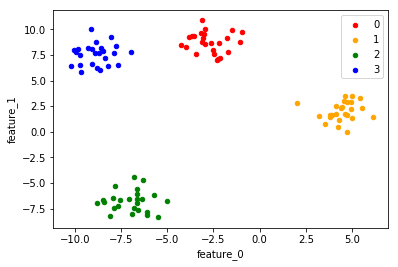
\includegraphics[width=0.65\textwidth]{./sync_imgs/datagen/blobs/2dimg.png}
\label{fig:datagen_blobs_2dimg}
\end{figure}

\textcolor{blue}{Data can also be generated in three (multiple) dimensions}

% {{{datagen_blobs_3dcode}}}
\begin{lstlisting}[style=pyInStyle]
X, y = datagen.make_blobs(centers=4, n_samples=100, n_features=3, random_state=42)
\end{lstlisting}

% {{{datagen_blobs_3dimg}}}
\begin{figure}
\centering
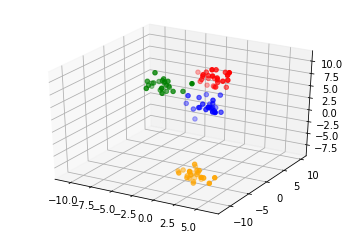
\includegraphics[width=0.65\textwidth]{./sync_imgs/datagen/blobs/3dimg.png}
\label{fig:datagen_blobs_3dimg}
\end{figure}

%\textcolor{blue}{More dataset types can be generated, the documentation can be found at (http://scikit-learn.org/stable/modules/classes.html#module-sklearn.datasets)}


\textcolor{blue}{see \textcolor{red}{local ref?} for more examples on how to generate data}



%%%%%%%%%%%%%%%%%%%%%%%% Data Pre-processing
\section{Data Preparation}

\textcolor{blue}{TODO: direct and indirect importance of datapreparation. indirect: feature engineering allows for more elegant and efficient solutions (e.g. calculating the time with a CNN of a clock face vs engineered features for the angles of the large and small hand.) }

\subsection{Data Pre-processing}

\textcolor{blue}{Data is rarely obtained in a form that is necessary for optimal performance of a learning algorithm. Data can be missing, can contain a mix of categorical and quantitative, can contain values on vastly different scales, etc.}

\textcolor{blue}{Building a good representation of your data -- feature extraction/engineering}

\textcolor{blue}{It is important to note that any parameters related to data pre-processing, such as feature scaling and dimensionality reduction, are obtained solely from observing the training set. The parameters for these methods obtained on the training set are then later applied to the test set. This is important since if these preprocessing parameters were obtained on the entire dataset and included the test set, the the model performance may be overoptimistic since then when applying the methods to the unseen data.}

\textcolor{blue}{make sure to use data that is relevant to the objective/problem.}

% TODO: case study example

\textcolor{blue}{make sure the data can be known at prediction time. e.g. will there be a delay between activity and being able to access that data at the data repository?}

% TODO: case study example

% TODO: expand
\textcolor{blue}{features should be numeric and have a meaningful magnitude (see below). In addition to being meaningful, the magnitude should be on a similar (small) range. e.g. if some data has one feature on a range 70,000-500,000 (estimated home value) and another feature on a 0-5 range (maybe number of bathrooms in a house), the higher values, in addition to being viewed as more meaningful (higher weights), large gradient updates may result that don't allow the network to converge (the updates are not fine grained enough).}

% TODO: case study example

\r{pre-processing may be used to reduce the dimensionality of the data, before training.}

\textcolor{blue}{make sure ``enough'' examples exist for the particular feature}

\textcolor{blue}{Don't mix magic values with values you already have. For example, if we have ratings 0-10, don't include a new column for rated vs not rated.}

\subsubsection{Handling Missing Data}

\paragraph{Filtering Out}

\textcolor{blue}{Simply removing any entries that are missing data. This is convenient and easy but may not be practical -- any time data is being removed, potentially useful information is lost and too much data may be removed.}

\textcolor{green}{TODO: Code in jupyter on how to do this with pandas and dropna -- key params - how, thresh, subset}

\paragraph{Filling In}

\textcolor{blue}{Estimating the missing data}

\subsubsection{Handling Categorical Data}

\paragraph{Encoding}

\textcolor{blue}{It may seem intuitive to represent categorical data with an integer value. However, this may not always be best. Let's pretend we're representing United States with arbitrary integer values and we assign values alphabetically; Alabama: 0, Alaska: 1, Arizona: 2, Arkansas: 3, California: 4, ..., Wisconsin: 48, Wyoming: 49. So far so good. \textcolor{red}{However, these values indirectly imply a relationship (that may not actually exist)} -- and imply that some states are more similar to one another than others (for instance, this encoding seemingly indicates that Alabama as most related to Alaska.) }

\textcolor{blue}{{one-hot encoding}\index{one-hot encoding} or one-of-k encoding\index{one-of-k encoding} is a method of encoding which represents each explanatory variable as a binary feature}

\textcolor{blue}{one-hot encoding reduces the relationship}

\textcolor{green}{TODO: show example of one hot encoding}

\textcolor{blue}{will lead to {sparse vectors}\index{sparse vectors} -- high dimensional vectors. This is memory intensive (some libraries have methods to address this --- SciPy and Pandas).}

\subsubsection{Feature Scaling, Normalization}

% TODO: this section needs to be restructured to present ideas in a logical flow/building on one another and the cost(time)/benefit

\textcolor{blue}{Ensuring variables exist on a similar scale and variance is important. If one variable is orders of magnitude larger than others, the variable may dominate the learning algorithm and prevent influence from the other variables.}

\textcolor{blue}{Generally would like to get each feature into the $-1 \le X_i \le 1$ or the $-0.5 \le X_i le 0.5$ range.}

\textcolor{blue}{"OK" if not exact, different people have different rules of thumb for when it is necessary to scale a feature into this range.}

\textcolor{blue}{Additionally, some learning algorithms converge more slowly.}

% hard clipping/capping

% log scalling -- good for when the data has a huge range

% TODO: Give an example


\paragraph{Mean Normalization}

\textcolor{blue}{feature $x$ is replaced by $x - \mu$ to create a zero mean}

% TODO: 2D figure showing a circle vs oval contour plot and how gradient descent may take longer on the "oval"

\paragraph{Min-Max scaling (Normalization)}

\textcolor{blue}{values are shifted and rescaled so they end up on a [0,1] range}

\paragraph{Standardization}

\textcolor{blue}{(Eq.~\ref{eq:preprocess_standardization}) first, subtract the sample mean, then divide by standard deviation variance}

\textcolor{blue}{pros: unlike min-max, not bound to specific range}

\textcolor{blue}{standardized values always have a zero mean and unit variance, a standard deviation of 1.}

\textcolor{blue}{gives our data the property of a standard normal distribution}

\begin{equation}
{X' = \frac{X - \mu}{\sigma}}
\label{eq:preprocess_standardization}
\end{equation}

\textcolor{green}{TODO: create code sample - numpy, and sklearn methods}

\subparagraph{Robust Scaler}

\textcolor{blue}{In order to reduce the effect of large outliers, a \textcolor{blue}{RobustScalar} may be used. Rather than subtract the mean and divide by the standard deviation, the median is subtracted and then the data is divided by the {interquartile range}\index{interquartile range} -- \textcolor{red}{see local ref?}}


\subsubsection{Others}

\paragraph{Removing Duplicates}

\paragraph{Outliers}

\textcolor{blue}{rather than remove outliers, the values may be capped.}
% TODO: example, in the California housing data, there are datapoints with 50 rooms per house

\paragraph{Discretization and Binning}

\textcolor{blue}{An example for this may be housing prices and latitude.}

% ? tf.feature_column.bucketized_column

\textcolor{blue}{rather than store a floating point, bins could be created. would like to keep the information (latitude may be useful, but the magnitude here is not useful (even if normalized) and so binning may be a great option)}

% TODO: figure for latitude (housing prices) and values pre/post binning

\subsubsection{Where to do preprocessing}

\textcolor{blue}{1. at execution time/with the TF graph}
\textcolor{blue}{2. apache beam ``in front'' of the graph (can use time windows)}
\textcolor{blue}{3. }



\textcolor{blue}{Batch vs Streaming}

% calculating rolling average

\subsubsection{Feature Engineering}

\textcolor{blue}{feature engineering is the process of altering the values of the data such that the problem becomes easier to solve as a result of expressing the data in a simplier/more relevant way. this usually required domain knowledge.}

\textcolor{green}{TODO: p.102 of Keras book fchollete uses a clock example that is very nice.}

%%%%%%%%%%%%%%%%%%%%%%%% Data Type Considerations + Feature Extraction
\section{Feature Extraction from Various Datatypes}

\textcolor{green}{TODO: Feature Extraction}


\subsection{Images}

\textcolor{green}{TODO: Images}


\subsubsection{Video}

\textcolor{green}{TODO: Video}


\subsection{Natural Language}

\textcolor{green}{TODO: Natural Language}

\subsubsection{Terminology}

\textcolor{blue}{A {corpus}\index{corpus} is a collection of documents. {vocabulary}\index{vocabulary} is a corpus's unique words}

\subsubsection{Pre-processing}

\textcolor{green}{TODO: Pre-processing}

\textcolor{blue}{converting all letters to lowercase}

\textcolor{blue}{stemming and lemmatization --- Condensing word forms (derived and inflected) into a single feature. These methods are used to reduce the dimensionality of the features space.}

\paragraph{Stop Word Filtering}

\textcolor{blue}{todo: removing words that are common throughout the language as well as potentially to most of the documents in a corpus. Typically stop words do not convey meaning through their meaning, but rather through their grammatical meaning.}

\paragraph{Tokenization}

\textcolor{blue}{Tokenization is the process of splitting and grouping characters together into meaningful sequences. \textcolor{red}{If a document is tokenized, the result is a set of tokens (words).} Tokens are not limited to words however, and may also be shorter sequences like punctuation characters and affixes.}

\textcolor{green}{TODO: Tokenization example}

\paragraph{Lemmatization}

\textcolor{green}{TODO: Lemmatization. converting words into their base form --- determining the lemma (morphological root) of an inflected word.}

\paragraph{Stemming}

\textcolor{green}{TODO: Stemming. There exist many stemming algorithms. Stemming removes all character patterns that appear to be affixes to a word. Note: the resulting word may or may not be a valid word e.g. \textcolor{red}{XXXXXXXX}.}

\subparagraph{Porter Stemming}

\subsubsection{Encoding}

\paragraph{Encoding Methods}

\subparagraph{Bag-of-Words}

\textcolor{blue}{{bag-of-words}\index{bag-of-words} similar to one-hot-encoding, it encodes words that appear in text as one feature for each word of interest. Does not encode any other information like syntax, grammar, or order of the words.}

\textcolor{blue}{Bag-of-Words encodes the corpus's vocabulary as a feature vector to represent each document. The intuition for using bag-of-words is that documents that contain similar words are likely to be similar to one another.}


\paragraph{tf-idf}

\textcolor{green}{TODO: tf-idf\index{tf-idf} (Eq.\ref{eq:tf_idf_def}) Inverse Document Frequency is a measure of how common/rare a term is in a corpus --- explain importance}

\begin{equation}
{log\frac{N}{1|XXXXXXXXTODOXXXXXXXXXX|}}
\label{eq:tf_idf_def}
\end{equation}

\subsubsection{Embedding}

\subparagraph{glove}

\textcolor{green}{TODO: glove}

\subparagraph{word2vec}

\textcolor{green}{TODO: word2vec}

\subsubsection{Other Notes}

% 'hashing trick' --- see p59 of Mastering ML with SKL

\subsection{Audio}


\textcolor{green}{TODO: Audio}



%%%%%%%%%%%%%%%%%%%%%%%% Data sampling and partitioning
\section{Partitioning Data}

\textcolor{blue}{Ideally, a model will generalize well i.e. a model will perform well on data that it has never seen. When evaluating a model, the performance is reported on a data that has never been seen by the model. When a dataset is obtained, one of the first steps performed is to partition the dataset -- a portion of the dataset is removed and placed aside as the ``test'' set that will later be used to measure the performance of an indicated model.}

\subsection{Types of Splits}

\textcolor{blue}{A learning method is trained on a collection of examples called the ``training set''. The performance of the learning method is then evaluated on another collection of examples known as the ``test set''. It is important to ensure that none of the instances in the test set are included in the training set -- a point that will be mentioned many times throughout this text. If the test set were to include examples from the training set, evaluating the whether the learning method has memorized the training set or generalizes well will be difficult.}

\textcolor{blue}{An additional set, known as the validation is typically used. The validation set is used to tune the hyperparameters of the learning algorithm and help prevent overfitting to the training data. Though the model does not train directly on the validation dataset (exception being when using k-folds cross validation) it is still possible to overfit the validation set since we are manually adjusting the hyperparameters to give the best result on the validation set. This situation is related to the concept of {information leaks}\index{information leaks} --- some information from the validation data \textit{leaks} into the model by tuning hyperparameters with regard to this information. This will generally lead to a  model that performs artificially well on the validation set (since this is what was optimized for)}

\textcolor{blue}{Along these same lines, it should be noted that evaluating on the test set should only be performed \textbf{once}.\textcolor{red}{this is important}. Otherwise, the model will be tuned to the test set, resulting in overly optimistic results. To compare different design choices to one another, it is best to compare and finalize them based on their performance on the validation set, before ``locking'' the model and evaluating its performance on test set.}

\begin{figure}[htp]
	\centering
	\includegraphics[width=0.5\textwidth]{example-image-a}\hfil
	\caption{Figure showing when to save best parameters (plus link to ``early stopping''), \textcolor{green}{TODO}}
	\label{fig:sample_split_save_best_params}
\end{figure}

\textcolor{blue}{There are no hard rules that clearly define how a dataset should be divided into training, validation, and test sets and usually the ratio of data in each split depends on the overall size of the dataset.}

\textcolor{blue}{Some common dataset splits (training:validation:test) are 50:20:30 and 40:20:40}

\begin{figure}[htp]
	\centering
	\includegraphics[width=0.5\textwidth]{example-image-b}\hfil
	\caption{Figure showing hold and common dataset splits, \textcolor{green}{TODO}}
	\label{fig:sample_split_hold_out}
\end{figure}

\textcolor{blue}{``hold out'' split}

\textcolor{blue}{{lucky split}\index{lucky split} is used to describe an instance in which, by chance, the test set contains easily predicted instances and the training set includes difficult to predict instances.}

\textcolor{blue}{Typically the performance of a machine learning algorithm improves with the number of training instances. However, quality is superior to quantity, in that a lot of ``bad'' data is worse than a smaller amount of ``good'' data -- in this sense, machine learning algorithms follow the ``garbage in, garbage out''.}



\subsection{k-Fold Cross Validation}

\r{cross validation is a method used to train across the entire training dataset without holding out an explicit validation set. The training data is partitioned, into $k$ ``folds'', and the algorithm is trained on all but one of these partitions and evaluated on the remaining partition. The partitions are then rotated such that each fold/partition is included in the training and evaluation of the algorithm. After sufficient training, (as defined by the individual), the model is then evaluated on the test set.}

\TD{stratfied k-fold cross validation}

\begin{figure}[htp]
	\centering
	\includegraphics[width=0.5\textwidth]{example-image-a}\hfil
	\caption{Figure showing how k-fold cross validation works, \textcolor{green}{TODO}}
	\label{fig:sample_split_k_fold}
\end{figure}

\subsubsection{k-Fold Validation with shuffling}

\textcolor{blue}{shuffle the data before splitting it k-ways --- where k-fold validation is performed multiple times}

% TODO: design a warn/caution/watch-out box
\textcolor{green}{WARN: every time you fold in the data/train on the data, the ``information leak'' is greater -- leading to likely overfitting}

\subsection{Sampling}

\textcolor{blue}{Things to consider when performing splits. How representative your data is -- compared to the population and compared to each split.}

\paragraph{Representative Data}

\begin{figure}[htp]
	\centering
	\includegraphics[width=0.5\textwidth]{example-image-b}\hfil
	\caption{Figure showing importance of shuffling data. one figure where the data isn't shuffled well and a split leads to a case where one split contains only a subset of the classes (not all the classes) \textcolor{green}{TODO}}
	\label{fig:sample_split_shuffle_importance}
\end{figure}

\textcolor{blue}{NOTE/WARN: only perform shuffling when it makes sense --- e.g. shuffling time series data would not be wise.}

\textcolor{blue}{WARN: It would be smart to check your data for any points where the same instance is included across both splits training/validation/test. If the dataset contains multiple samples of the same instance, and they are inluded in different splits, there is now redundancy and even worse: imagine a situation in which the same instance (e.g. the same image or an image of the same object, just at a different angle) we now are training on our test set!  Bottom line: it is important to ensure the training, validation, and test sets are all disjoint.}

\paragraph{Representative Data}

\textcolor{blue}{Random vs \textcolor{red}{stratified}}

\TD{Stratified -- preserves ratio}


\section{Some Terms}

\emph{input variable(s)} -- predictors, independent variables, features, regressors, controlled variables, exposure variables or simply variables.
 
\emph{output variable(s)} -- response or dependent variable. May also be known as regressands, criterion variables, measured variables, responding variables, explained variables, outcome variables, experimental variables, labels.

\textcolor{blue}{Both input and output variables may take on continuous or discrete values.}

\emph{relationship} $Y = f(x) + \epsilon$ \textcolor{blue}{estimate $f$. prediction and inference}.

\textcolor{blue}{\emph{reducible error\index{reducible error}} -- the estimated function $\hat{f}$ will likely not be perfect, and the reducible error is the error that could be corrected.  The \emph{irreducible error} is an error that can not be corrected. The irreducible error may be larger than zero due to \emph{unmeasured variables} \emph{e.g.} varibles that were not measured and \emph{unmeasurable variation} \emph{e.g.} an individual's feelings/emotions or variation in the production of a product. The irreducible error provides an upper bound on the performance of the predicted $\hat{f}$}

\section{Type of Learning}

\textcolor{blue}{Three main types of machine learning: supervised, unsupervised, and reinforcement.}

% From ML for Predictive Data Analytics
\textcolor{blue}{Another way to group types of learning -- Information-based, similarity-based, probability-based, and error-based}

\subsection{Supervised}

\textcolor{blue}{observe input variables with corresponding output values. A program that predicts an output for a in input by learning from pairs of labeled inputs and outputs. Classification \textcolor{red}{ref} and regression \textcolor{red}{ref} are subcategories of supervised learning}

\subsection{Unsupervised}

\textcolor{blue}{observe input variables without corresponding output values and attempts to discover patterns in the data.}

% p14 of mastering ml agorithms
\textcolor{blue}{There is no error signal to measure, rather, performance metrics report some attribute of structure discovered in the data, such as the distances within and between clusters.}
 
% clustering
\subsubsection{Clustering}

\textcolor{blue}{Finding sub groups where observations are more similar to eachother based on some similarity measure. Clustering is sometimes referred to as ``unsupervised classification'' and is often used to explore a dataset.}

\textcolor{blue}{An example of clustering may be to group a collection of documents into categories, or songs into genres.}

% principal components
\subsubsection{Dimensionality Reduction}

\textcolor{blue}{where the goal is to reduce the dimensionality of the data while retaining as much as the relevant information as possible}

\textcolor{blue}{A high number of features may be computationally costly. Ability to generalize may be reduced if some of the features capture noise or are irrelevant to the underlying relationship. The goal could be to find the features that account for the greatest changes in the response variable}


\subsection{Semi-supervised Learning}

\textcolor{blue}{`semi-supervised learning', another type of learning, makes use of both supervised and unsupervised data.}

\subsection{Reinforcement}

\textcolor{blue}{Reinforcement learning does not learn from labeled pairs of inputs and outputs, rather it learns from `feedback' from decisions that are not explicitly corrected.}

\textcolor{blue}{Goal -- develop an \emph{agent} that improves it's performance based on interactions with an \emph{environment} based on a \emph{reward}}

\subsection{Supervised vs Unsupervised}

\subsection{Classification vs Regression}

\subsubsection{Regression} 

Regression, also called regression analysis \textcolor{red}{local ref?} involves predicting a continuous or quantitative output value. For example attempting to find a relationship between a given predictor/explainatory variables (age, job title, zip code) and a continuous response (an individuals outcome).

\subsubsection{Classification} 

Classification involves predicting categorical (discrete) or qualitative output value (such as a non-numerical value). 

\textcolor{blue}{Binary classification (benign vs malignant) and multi-class classification (identifying many different skin diseases).}

\subsection{Multi-label classification}
\textcolor{blue}{TODO: {multi-label classification}\index{multi-label classification} --- where a classifier assigns multiple labels to each instance}


\subsubsection{Approaches: Problem transformation}

\textcolor{blue}{There are two main approaches to multi-label classification}

\textcolor{blue}{{Problem transformation}\index{Problem transformation} modify the original multi-label problem to a set of single-label classification problems.}

\paragraph{Unique set/combination of labels}

\textcolor{green}{TODO: table and example.}

\textcolor{blue}{Two main concerns with this methodology: i) increasing the number of classes is impractical and will often have very few instances and ii) the classifier can only predict combinations that were seen in the training data.}

\paragraph{Many Binary Classifiers}

% p124[112] of Mastering ML with SKL
\textcolor{blue}{Train a classifier for each label in the training set. The final prediction is the combination of all the predictions from the binary classifiers.}

\textcolor{blue}{The main concern with this approach is that the relationships between labels is ignored.}

\subsubsection{Evaluating Multi-label Classification}

\textcolor{blue}{see \textcolor{red}{local ref}.}

% page 94 of AGtext
One-versus-all \emph{OvA} (also \emph{one-versus-rest}) -- 

One-versus-one (OvO) -- train a binary classifier for every pair


\textcolor{blue}{Binary classification can be extended to multi-class classification via the OvR method.}

%\subsubsection{Bayes Classifier}

\section{Training}

\section{Quality of Fit}

%% regression example

\subsection{Regression Example}

\textcolor{blue}{Mean Squared Error.$\hat{f}(x_i)$ is the prediction that $\hat{f}$ produces for the $i$th sample. The output will be small for predicted values that are similar to the ground truth}

\begin{equation}
{MSE = \frac{1}{n}\sum_{i=1}^{n}(y_i - \hat{f}(x_i))^2}
\label{eq:MSE_def}
\end{equation}

%% classification example

\subsection{Classification Example}

\textcolor{blue}{The proportion of mistakes that are made.}

\begin{equation}
{error\_rate = \frac{1}{n}\sum_{i=1}^{n}(y_i \ne \hat{y_i})}
\label{eq:class_error_rate_def}
\end{equation}

\textcolor{blue}{$\hat{y_i}$ is the predicted classification label for the $i$th observation using our predictor/model $\hat{f}$ and $y_i$ is the ground truth label}

\section{(Over$|$Under)fitting}

\subsection{Overfitting}

\textcolor{blue}{Overfitting\index{Overfitting} refers to a case in which a model fits the training data very well but does not fit validation/test set. If a model is overfitting, it is said to have a high variance and is analogous to memorizing the training set.}

\textcolor{blue}{Overfitting can arise from modeling data with too many parameters/too complex of a model.}

\textcolor{green}{TODO: figure showing an example of overfitting}

\subsection{Underfitting}

\textcolor{blue}{Underfitting\index{Underfitting} refers to a case in which a model does not fit the training data well. If a model is underfitting, it is said to have a high bias}

\textcolor{blue}{Underfitting can arise from modeling data with too few parameters/too simple of a model.}

\textcolor{green}{TODO: figure showing an example of underfitting}


\section{Bias Variance Trade-off}

\textcolor{blue}{Two fundamental causes of prediction error in a model -- the bias and the variance.}

\subsection{Variance}
\textcolor{blue}{variance\index{Variance} refers to the amount the model would change (consistency or variability) if it was re-trained/estimated multiple using a different subsets of the training data set. A model that has high variance is sensitive to randomness in the training data}

\textcolor{blue}{A model with high variance may be described as highly flexible and will likely overfit the data.}


\subsection{Bias}
\textcolor{blue}{Bias\index{Bias} refers to the amount of error that is introduced by approximating a problem with a model that is simpler than the (complex) problem}

\textcolor{blue}{A model with high bias will produce similar errors for instances regardless of the training data that is used to train the model -- the model is more strongly ``biased'' to its own assumptions of the relationship (as defined by the model), than the relationship the data may be indicating. A model with high bias may also be described as inflexible and will likely underfit the data.}


% not word-for-word, but example adapted from p35 of ISL
\textcolor{red}{For example, linear regression assumes a linear relationship between the features and labels. However, it is unlikely that a true linear relationship exists and so using linear regression to model this type of particular problem will likely introduce some bias.}

\subsection{Trade-Off}

% TODO: see page 34 of ISL for eq and explaination here

\textcolor{blue}{In general, as a more ``flexible'' model is used, the variance will increase and the bias will decrease.}


% see page 36 of ISL
\textcolor{blue}{It is easy to obtain a model with low bias but high variance (\emph{e.g.} drawing a squiggly line through every training observation) and it is easy to obtain a model with low variance but high bias (\emph{e.g.} drawing a straight line approximating every training observation) but it is difficult to obtain a model that has both low variance and low bias.}

\textcolor{blue}{It should be noted that in a real world example, it may not be possible to explicitly calculate the test error, bias, or variance.}

\textcolor{green}{TODO: para about using regularization here/finding the right balance \textcolor{red}{local ref to regularization?}}

\subsection{Parametric vs non-parametric}

\subsubsection{parametric}

\textcolor{blue}{parametric models are models that learn a fixed number of parameters, independent from the number of training instances, that able to classify new data points without requiring the original dataset anymore. First, a function form is selected (linear, polynomial, etc.), then the coefficients for the function are learned form the training data.}
	
\textcolor{blue}{Examples of parametric models may be simple artificial neural networks, naive bayes, logistic regression, etc.}

\subsubsection{nonparametric}

%% unsure about this! 
\textcolor{red}{Nonparametric models are not models without parameters, rather they are models were the number of parameters are not fixed, they may grow with the number of training instances}

\textcolor{blue}{An Example of a nonparametric model may be k-Nearest neighbors -- where the model does not assume anything about the form of the mapping function and makes predictions based on the k most similar training instances.}

\textcolor{blue}{A disadvantage to this type of approach is that the computational complexity for classifying new samples grow linearly with the number of samples in the training set.}

\textcolor{blue}{May be useful when little is known about the underlying relationship in the data and there is an abundance of data.}

\subsection{Eager vs Lazy Learners}

\textcolor{green}{TODO: Eager vs Lazy overview}
\textcolor{blue}{Training an eager learner is often more computationally expensive, but typically prediction with the resulting model is inexpensive.}

\subsubsection{Eager Learners}

\textcolor{blue}{Eager learners estimate the parameters of a model that generalize to a training set}

\subsubsection{Lazy Learners}

\textcolor{blue}{Also known as Instance-based Learners}

\textcolor{blue}{Lazy learners store the training dataset with little to no processing.}


\subsection{Generative vs Discriminative Models}

\textcolor{green}{TODO: Generative vs Discriminative models overview}
%\textcolor{blue}{}

\subsubsection{Generative Models}

\textcolor{green}{TODO: Generative Models}

\subsubsection{Discriminative Models}

\textcolor{green}{TODO: Discriminative Models}

\subsection{Strong vs Weak Learners}

\textcolor{green}{TODO: Strong vs Weak learners (classifier, predictor, etc.) overview}
%\textcolor{blue}{}

\subsubsection{Strong Learners}

\textcolor{green}{TODO: Strong Learners are models that are arbitrarily better than weak learners.}

\subsubsection{Weak Learners}

\textcolor{green}{TODO: Weak Learners are models (typically simple models) that perform only slightly better than random chance. }


\section{Online Learning}

% See p.246 of Understanding Machine learning
\textcolor{blue}{difference to \textcolor{red}{PAC learning?}}

\section{Ensemble Methods}

\textcolor{green}{TODO: overview - discussed in more detail in \textcolor{red}{local ref?}}

\section{Hyper-Parameters}

\subsection{Hyper-Parameter Optimization}

\subsubsection{Grid Search}

\textcolor{blue}{{Grid search}\index{Grid search} Exhaustive search that trains+evaluates a model for each combination of specified hyperparameter configurations and combinations defined by a Cartesian product of the sets of possible values for each hyperparameter.}

\subsubsection{Randomized Search}

\textcolor{blue}{{Randomized search}\index{Randomized search} }

\textcolor{green}{TODO: figure demonstrating difference between grid and randomized search}

\subsubsection{Other Methods}

\textcolor{blue}{See \textcolor{red}{local ref? --- advanced methods and research}}

%%%%%%%%%%%%%%%%%%%%%%%% Optimizers
\subsection{Optimizers}

\textcolor{blue}{Estimate the values of the model's parameters that minimize the value of the cost function}

\textcolor{blue}{"turning a loss function into a search strategy"}

\subsubsection{Gradient Descent}

\textcolor{blue}{Gradient Descent --- overview --- optimization algorithm that can be used to estimate the local minimum of a function}

\textcolor{blue}{Iteratively updates the model parameters by calculating the partial derivatives of the cost function at each step during training}

\textcolor{blue}{Gradient descent is only guaranteed to find the local minimum of the cost function.}

\textcolor{blue}{simultaneous update.}


\paragraph{Batch Gradient Descent}

\textcolor{blue}{batch gradient descent --- taking a step (update the weights) opposite (down) the gradient calculated from the entire training set}

\textcolor{blue}{Batch gradient descent is deterministic --- will produce the same paramter values if the same dataset is used multiple times.}


\paragraph{Stochastic Gradient Descent}

\textcolor{blue}{Stochastic Gradient Descent (sometimes called iterative or on-line gradient descent) --- rather than update the weights based on the sum of the accumulated errors, the weights are updated for each training sample}

\textcolor{blue}{Stochastic gradient descent is deterministic --- may produce the different parameter values if the same dataset is used multiple times. May not minimize the cost function as well as gradient descent but the approximation is often ``close enough''.}


\paragraph{Mini-batch Gradient Descent}

\textcolor{blue}{mini-batch gradient descent --- compromise between batch and stochastic gradient descent where the gradient is calculated over a batch of training data}

\textcolor{blue}{Since the gradient is calculated on a single example, the error surface will appear noisier than if it was calculated over a batch or the entire training set.}

\textcolor{blue}{When using stochastic gradient descent, it is important to shuffle the data after each epoch.}


% when looking at specific optimizers, http://ruder.io/optimizing-gradient-descent/ was a useful resource

\subsection{Improved Optimizers}

\textcolor{blue}{Some of the common optimizers are listed below. Additional optimizers are discussed in \textcolor{red}{local ref?}}

\subsubsection{Momentum}

\textcolor{blue}{Momentum~\cite{qian1999momentum}, will reduce the learning rate when the gradient is small}

\subsubsection{RMSProp}

\subsubsection{Nesterov}

\textcolor{blue}{Nesterov accelerated gradient (NAG)}

\subsubsection{Adam}

\textcolor{blue}{Adaptive Moment Estimation (Adam)~\cite{kingma2014adam}}


%%%%%%%%%%%%%%%%%%%%%%%%%%%%%%%%%%%%%%%%%%%%%%%%%%%%%%%%%%%%%%%%%%%%%%%%%%%%%%%%%%%%%%
%%%%%% TODO: Cut off -- these optimizers will be moved to another location (research?)
%%%%%%%%%%%%%%%%%%%%%%%%%%%%%%%%%%%%%%%%%%%%%%%%%%%%%%%%%%%%%%%%%%%%%%%%%%%%%%%%%%%%%%

\subsubsection{Nadam}

\textcolor{blue}{Nadam (Nesterov-accelerated Adaptive Moment Estimation)~\cite{dozat2016incorporating}}

\subsubsection{AdaGrad}

\textcolor{blue}{Adagrad~\cite{duchi2011adaptive}, will assign frequently occurring features low learning rates}

\subsubsection{AdaDelta}

\textcolor{blue}{Adadelta~\cite{zeiler2012adadelta}, expands on AdaGrad by avoiding reducing the learning rate to zero.}

\subsubsection{AdaMax}

\subsubsection{Ftrl}

\textcolor{blue}{``follow the regularized leader'', \textcolor{red}{CITE}, \textcolor{red}{works well on wide modes?}}







%%%%%%%%%%%%%%%%%%%%%%%% Evaluation
\section{Evaluation}

\r{Importance of dataset partitioning \textcolor{red}{local ref?}}

% \textcolor{blue}{The best performance measure will vary depending on the task. For instance, in a medical setting, it may be life threating to classify an event as ``healthy'' when the patient is not healthy.}

\r{A performance measure is used to capture, empirically, how well a prediction made by the model aligns with the expected, ground truth, value.}

\subsection{Creating a Test Set}

% rough para
\r{The most important rule regarding evaluating models, is to ensure that the data used to evaluate the model has never been used before to influence the during training or selection -- this means it was not used during training to update the parameters and it was not used to influence which models are `best' (like a validation set may be used for)}

\r{The performance of a model on a test set may be indicative of how well the model can generalize to unseen data. (This assumes your data sample is representative of the data population)}

\r{Hold-out test set -- created by randomly sampling the dataset. Again, it is important to emphasize that the instances in the test set are never used in the training process and are instead reserved for use only during the evaluation phase.}

\r{peeking\index{peeking}, is an issue that arises when part or all of the test set is included in the training set. This means the model has already seen the data on which the model will be evaluated and so it is possible, probable, that the model will produce high evaluation scores, which will likely translate to an overoptimistic estimation of the models performance when used in production.}

\r{Evaluating the performance of a model can be challenging and will vary depending on the task. For instance, accuracy may not always be the best measure of performance -- consider a medical setting in which sensitivity may be more important since a false negative may be life threatening where as a false positive may only require additional observation.}

\r{When comparing various models, it may be challenging to rank them on a single performance measure. \textcolor{green}{TODO: more.}}

\subsection{Qualitative Evaluation}

\r{generalization is a measure of how well the system preforms on previously unseen data.}

\subsubsection{(Over$|$Under)fitting and Capacity}

\r{{Model capacity}\index{model capacity} helps control how likely a model is to overfit or underfit. Where a model with low capacity may have difficulty fitting a a training set and a model with high capacity may ``overfit'' the data by essentially memorizing the training data.}

\r{Model capcity is closely related to model complexity and the models {hypothesis space}index{hypothesis space} (The set of functions available to the learning algorithm --- \textcolor{green}{TODO: expand - for example a linear vs polynomial model})}

\TD{TODO: figure showing training and validation error and 1) optimal capacity, 2) under and overfitting region 3)generalization gap, 4) capacity}

\paragraph{Overfitting}

\r{Overfitting\index{Overfitting} refers to a case in which a model fits the training data very well but does not fit validation/test set. If a model is overfitting, it is said to have a high variance and is analogous to memorizing the training set.}

\r{Overfitting can arise from modeling data with too many parameters/too complex of a model.}

\TD{TODO: figure showing an example of overfitting}

% addressing overfitting: 1) reduce number of features (manual selection or w/model selection algor) 2) regularization

\begin{figure}[htp]
	\centering
	\includegraphics[width=0.3\textwidth]{example-image-a}\hfil
	\includegraphics[width=0.3\textwidth]{example-image-b}\hfil
	\includegraphics[width=0.3\textwidth]{example-image-c}\hfil
	\caption{Figure example showing the same 2d dataset and an underfitting, overfitting, and ``good'' fitting. \textcolor{green}{TODO} circles=training, x=test -- include scores for each.. slight curve' under=linear, over=extreme poly, good=``smooth''}
	\label{fig:basics_eval_fitting_examples}
\end{figure}

\paragraph{Underfitting}

\r{Underfitting\index{Underfitting} refers to a case in which a model does not fit the training data well. If a model is underfitting, it is said to have a high bias}

\r{Underfitting can arise from modeling data with too few parameters/too simple of a model.}

\TD{TODO: figure showing an example of underfitting}


\subsubsection{Bias Variance Trade-off}

\r{Two fundamental causes of prediction error in a model -- the bias and the variance.}

\paragraph{Variance}
\r{variance\index{Variance} refers to the amount the model would change (consistency or variability) if it was re-trained/estimated multiple using a different subsets of the training data set. A model that has high variance is sensitive to randomness in the training data}

\r{A model with high variance may be described as highly flexible and will likely overfit the data.}


\paragraph{Bias}
\r{Bias\index{Bias} refers to the amount of error that is introduced by approximating a problem with a model that is simpler than the (complex) problem}

\r{A model with high bias will produce similar errors for instances regardless of the training data that is used to train the model -- the model is more strongly ``biased'' to its own assumptions of the relationship (as defined by the model), than the relationship the data may be indicating. A model with high bias may also be described as inflexible and will likely underfit the data.}


% not word-for-word, but example adapted from p35 of ISL
\textcolor{red}{For example, linear regression assumes a linear relationship between the features and labels. However, it is unlikely that a true linear relationship exists and so using linear regression to model this type of particular problem will likely introduce some bias.}

\paragraph{Trade-Off}

% TODO: see page 34 of ISL for eq and explaination here

\r{In general, as a more ``flexible'' model is used, the variance will increase and the bias will decrease.}

\r{One reason to choose a more restrictive model is that they are often more interpretable.}

\begin{figure}[htp]
	\centering
	\includegraphics[width=0.4\textwidth]{example-image-a}\hfil
	\includegraphics[width=0.4\textwidth]{example-image-b}\hfil
	\caption{\TD{side by side figure: a: complex vs simple training on trainnig data (nth poly vs linear), b: same models on test data}}
	\label{fig:basics_eval_tradeoff_examples}
\end{figure}


% see page 36 of ISL
\r{It is easy to obtain a model with low bias but high variance (\emph{e.g.} drawing a squiggly line through every training observation) and it is easy to obtain a model with low variance but high bias (\emph{e.g.} drawing a straight line approximating every training observation) but it is difficult to obtain a model that has both low variance and low bias.}

\textcolor{blue}{It should be noted that in a real world example, it may not be possible to explicitly calculate the test error, bias, or variance.}



\begin{figure}[htp]
	\centering
	\includegraphics[width=0.3\textwidth]{example-image-a}\hfil
	\includegraphics[width=0.3\textwidth]{example-image-b}\hfil
	\includegraphics[width=0.3\textwidth]{example-image-c}\hfil
	\caption{\TD{same 2D dataset with 3 layers and the hidden layer in a has few nodes, b: normal amount of nodes, and c: many nodes} \r{illistrative that the number of connections and complexity increases the chances for overfitting also increases}}
	\label{fig:basics_eval_nodesinhidden}
\end{figure}


\begin{figure}[htp]
	\centering
	\includegraphics[width=0.2\textwidth]{example-image-a}\hfil
	\includegraphics[width=0.2\textwidth]{example-image-b}\hfil
	\includegraphics[width=0.2\textwidth]{example-image-c}\hfil
	\includegraphics[width=0.2\textwidth]{example-image-a}\hfil
	\caption{\TD{same 2D dataset with one, two, three and four hidden layers}}
	\label{fig:basics_eval_numlayers}
\end{figure}

\r{observing a direct trade-off between overfitting and model complexity.}

\r{When we talk about deep learning, we're talking about deep and powerful models that are attempting to solve complex problems that are prone to overfitting and thus usually employ additional countermeasures, such as regularization, to help prevent overfitting.}


\TD{TODO: para about using regularization here/finding the right balance \textcolor{red}{local ref to regularization?}}



%%%%%%%%%%%%%%%%%%%%%%%% Metrics
\subsection{Metrics}

\textcolor{green}{TODO: talk about metrics/streaming metrics -- mention contrib}

